% \documentclass{article}
\documentclass[tikz]{standalone}
\usepackage{tikz}
\usetikzlibrary{shapes.geometric, arrows.meta}

\tikzstyle{startstop} = [rectangle, rounded corners, minimum width=4cm, minimum height=1cm, text centered, draw=black, fill=gray!20]
\tikzstyle{process} = [rectangle, minimum width=4.3cm, minimum height=1cm, text centered, draw=black, fill=blue!10]
\tikzstyle{parallel} = [rectangle, minimum width=4.3cm, minimum height=1cm, text centered, draw=black, fill=green!10]
\tikzstyle{decision} = [diamond, aspect=2.2, text centered, draw=black, fill=orange!20]
\tikzstyle{arrow} = [thick,->,>=stealth]

\begin{document}
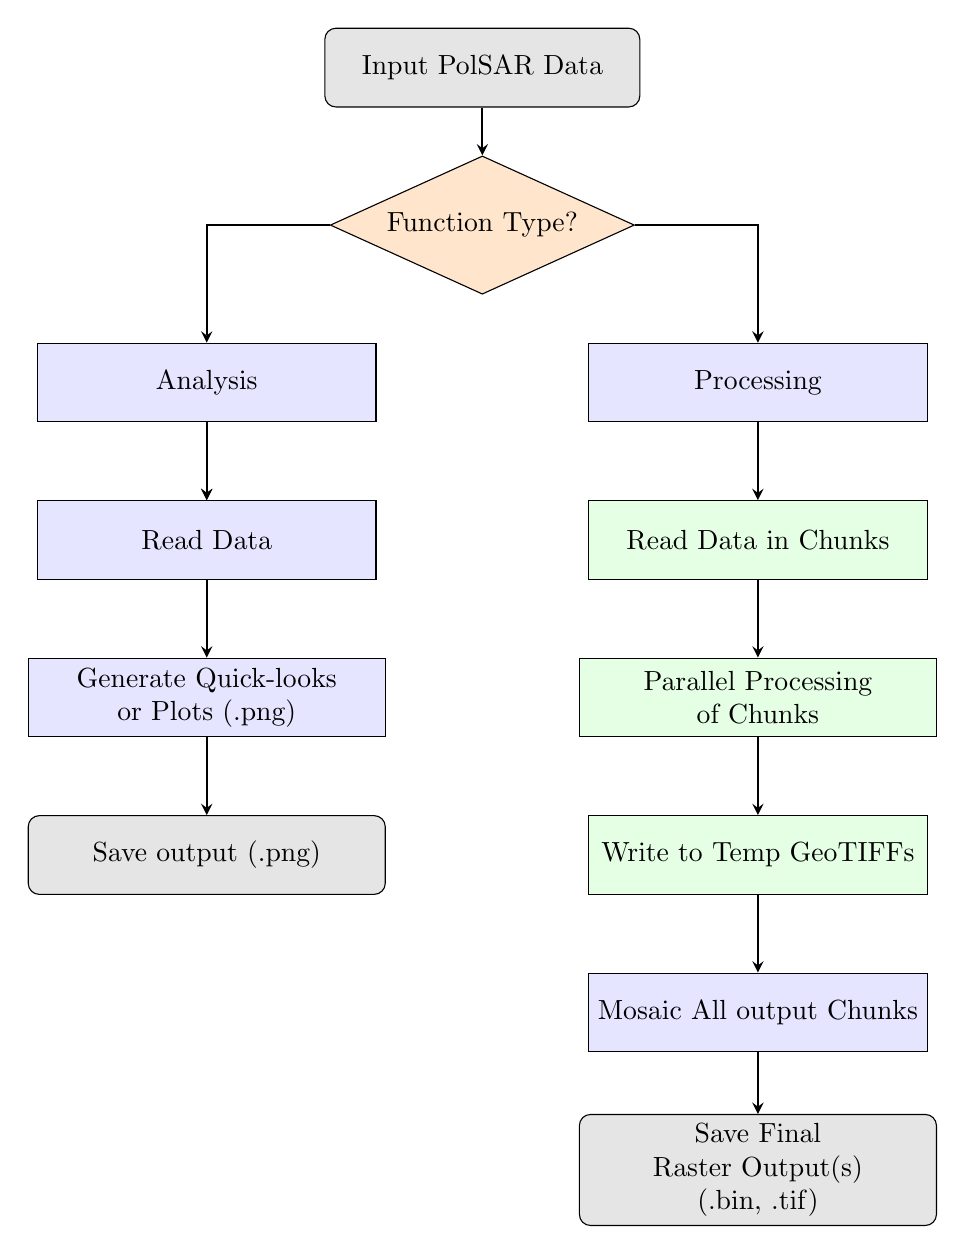
\begin{tikzpicture}

% Nodes
\node (start) at (3,0) [startstop] {Input PolSAR Data};
\node (decide) at (3,-2) [decision] {Function Type?};

\node (analysis) at (-0.5,-4) [process] {Analysis};
\node (readplot) at (-0.5,-6) [process] {Read Data};
\node (genplot) at (-0.5,-8) [process,text width=4.3cm, align=center] {Generate Quick-looks\\or Plots (.png)};
\node (saveplot) at (-0.5,-10) [startstop,text width=4.3cm, align=center]{Save output (.png)};


\node (processing) at (6.5,-4) [process] {Processing};
\node (chunk) at (6.5,-6) [parallel] {Read Data in Chunks};
\node (parallelproc) at (6.5,-8) [parallel,text width=4.3cm, align=center] {Parallel Processing\\ of Chunks};
\node (tempgeotiff)at (6.5,-10)  [parallel] {Write to Temp GeoTIFFs};
\node (mosaic) at (6.5,-12) [process] {Mosaic All output Chunks};
\node (save)at (6.5,-14)  [startstop,text width=4.3cm, align=center] {Save Final Raster Output(s)\\(.bin, .tif)};

% Arrows
\draw [arrow] (start) -- (decide);
\draw [arrow] (decide.west)  -| (analysis.north);
\draw [arrow] (decide.east)-|  (processing.north);

\draw [arrow] (analysis) -- (readplot);
\draw [arrow] (analysis) -- (readplot);
\draw [arrow] (readplot) -- (genplot);
\draw [arrow] (genplot) -- (saveplot);


\draw [arrow] (processing) -- (chunk);
\draw [arrow] (chunk) -- (parallelproc);
\draw [arrow] (parallelproc) -- (tempgeotiff);
\draw [arrow] (tempgeotiff) -- (mosaic);
\draw [arrow] (mosaic) -- (save);



\end{tikzpicture}
\end{document}
